\section{Аналитическая часть}

\subsection{Анализ задачи и существующих решений}

Необходимо разработать программу для отображения информации о репетиционных базах с возможностью для музыканта бронировать или отменять свои репетиции, а для владельца реп. базы - отслеживать записи на свою реп. базу.

На сегодняшний день существует всего два подобных приложения:
\begin{itemize}
	\item MUSbooking
	
	Это наиболее известное и популярное приложение по бронированию творческих площадок.
	
	Его основные преимущества: возможность бронирования любых творческих площадок и возможность бронирования в других городах России (не только в Москве).
	
	Основной недостаток: нельзя посмотреть сразу весь список зарегистрированных реп. баз в текущем городе. Список доступных реп. баз можно посмотреть только после указания конкретного времени репетиции, что крайне неудобно в определённых ситуациях.
	
	\item TONESKY
	
	Основное преимущество: возможность заранее посмотреть весь список зарегистрированных реп. баз.
	
	Из недостатков: отсутствие поиска по реп. базам, отсутствие цены на превью (т. е., чтобы посмотреть цену, надо зайти «вглубь» и посмотреть подробную информацию), ориентация только на Москву (не существенно в рамках моей задачи).
\end{itemize}

\subsection{Формализация данных}

База данных должна хранить информацию о:

\begin{itemize}
	\item репетиционной базе и её комнатах;
	\item оборудовании;
	\item пользователях (музыкантах и владельцах) и об их забронированных репетициях или реп. базах соответственно.
\end{itemize}

\begin{figure}[h!]
	\begin{center}
		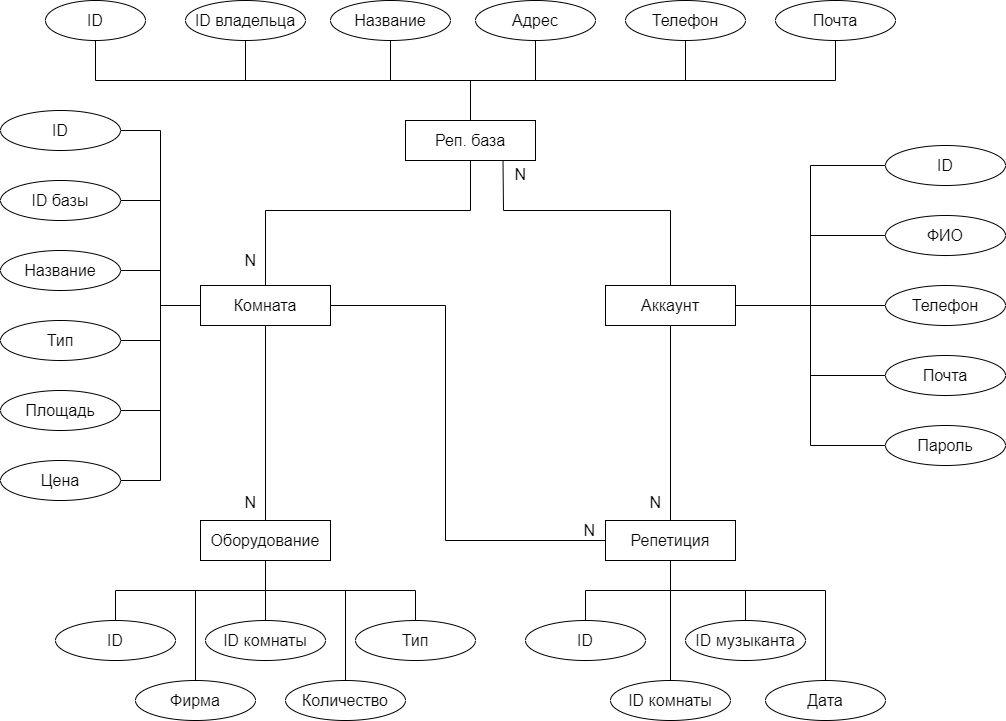
\includegraphics[scale=0.45]{inc/img/ER_Chena.png}
	\end{center}
	\captionsetup{justification=centering}
	\caption{ER-диаграмма разрабатываемой базы данных}
	\label{img:er-diagram}
\end{figure}

\begin{table}[!h]
	\captionsetup{justification=centering}
	\caption{\label{tab:data} Категории и сведения о данных}
	\begin{center}
		\begin{tabular}{|p{0.2\textwidth}|p{0.7\textwidth}|}
			\hline
			\textbf{Категория} & \textbf{Сведения}\\
			\hline
			Реп. база & Название, адрес, телефон, почта, кому принадлежит \\
			\hline
			Комната & Название, тип (вокал/группа и т. д.), площадь, стоимость за 3 часа, к какой репбазе относится \\
			\hline
			Оборудование в комнате & Тип (усилитель/ударные/микрофон и т. д.), бренд, количество, к какой комнате относится \\
			\hline
			Аккаунт & ФИО, телефон, почта \\
			\hline
			Репетиция & Время, какой музыкант (аккаунт), какая комната \\
			\hline
		\end{tabular}
	\end{center}
\end{table}

\newpage

\subsection{Типы пользователей}

Из задачи ясно, что есть два типа пользователей: обычный музыкант и владелец реп. базы. Помимо этого, будет также выделена роль администратора приложения. Для всех троих будет нужна авторизация.

\begin{figure}[h!]
	\begin{center}
		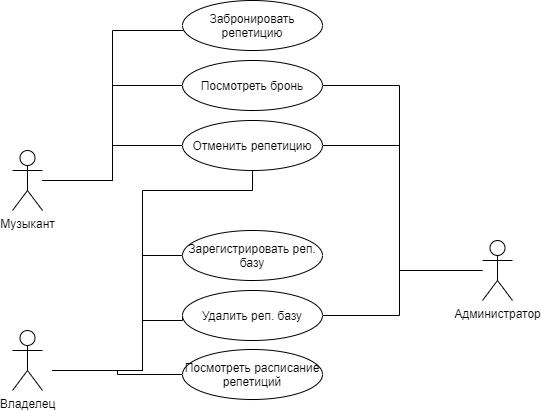
\includegraphics[scale=0.7]{inc/img/Use-Case.png}
	\end{center}
	\captionsetup{justification=centering}
	\caption{Use-case диаграмма приложения}
\end{figure}

\begin{table}[!h]
	\captionsetup{justification=centering}
	\caption{Типы пользователей и их полномочия}
	\begin{center}
		\begin{tabular}{|p{0.25\textwidth}|p{0.65\textwidth}|}
			\hline
			\textbf{Тип пользователя} & \textbf{Полномочия}\\
			\hline
			Музыкант & Бронирование репетиций, отмена репетиций, просмотр брони \\
			\hline
			Владелец & Добавление репбазы, удаление своей репбазы, просмотр записей на репетиции, отмена репетиций \\
			\hline
			Администратор & Удаление репбазы, отмена репетиций, просмотр бронирований \\
			\hline
		\end{tabular}
	\end{center}
\end{table}

\subsection{Классификации СУБД}

Система управления базами данных (СУБД) – совокупность программных и лингвистических средств общего или специального назначения, обеспечивающих управление созданием и использованием баз данных \cite{subd_opr}.

Основными функциями СУБД являются:
\begin{itemize}
	\item управление данными на внешней памяти;
	\item управление данными в оперативной памяти с использованием дискового кэша;
	\item журнализация изменений, резервное копирование и восстановление базы данных после сбоев;
	\item поддержка языков БД.
\end{itemize}

\textbf{Классификации СУБД:}

По модели данных:
\begin{itemize}
	\item дореляционные;
	
	\textbf{Иерархические.} Это модель данных, где используется представление базы данных в виде древовидной (иерархической) структуры, состоящей из объектов (данных) различных уровней.
	
	\textbf{Сетевые.} Это логическая модель данных, являющаяся расширением иерархического подхода, строгая математическая теория, описывающая структурный аспект, аспект целостности и аспект обработки данных в сетевых базах данных.
	
	Разница между иерархической моделью данных и сетевой состоит в том, что в иерархических структурах запись-потомок должна иметь в точности одного предка, а в сетевой структуре данных у потомка может иметься любое число предков.
	
	\item реляционные.
	
	Реляционная модель данных является совокупностью данных и состоит из набора двумерных таблиц. При табличной организации отсутствует иерархия элементов. Таблицы состоят из строк – записей и столбцов – полей. На пересечении строк и столбцов находятся конкретные значения. Для каждого поля определяется множество его значений. За счет возможности просмотра строк и столбцов в любом порядке достигается гибкость выбора подмножества элементов.
	
	Реляционная модель является удобной и наиболее широко используемой формой представления данных.
	
\end{itemize}

Модель данных — это абстрактное, самодостаточное, логическое определение объектов, операторов и прочих элементов, в совокупности составляющих абстрактную машину доступа к данным, с которой взаимодействует пользователь. Эти объекты позволяют моделировать структуру данных, а операторы — поведение данных \cite{data_model}.

По степени распределённости:
\begin{itemize}
	\item локальные (все части локальной СУБД размещаются на одном компьютере);
	\item распределённые (части СУБД могут размещаться не только на одном, но на двух и более компьютерах).
\end{itemize}

По способу доступа к БД:
\begin{itemize}
	\item файл-серверные;
	
	В файл-серверных СУБД файлы данных располагаются централизованно на файл-сервере. СУБД располагается на каждом клиентском компьютере (рабочей станции). Доступ СУБД к данным осуществляется через локальную сеть. Синхронизация чтений и обновлений осуществляется посредством файловых блокировок.
	
	Преимуществом этой архитектуры является низкая нагрузка на процессор файлового сервера.
	
	Недостатки: потенциально высокая загрузка локальной сети; затруднённость или невозможность централизованного управления; затруднённость или невозможность обеспечения таких важных характеристик, как высокая надёжность, высокая доступность и высокая безопасность. Применяются чаще всего в локальных приложениях, которые используют функции управления БД; в системах с низкой интенсивностью обработки данных и низкими пиковыми нагрузками на БД.
	
	На данный момент файл-серверная технология считается устаревшей, а её использование в крупных информационных системах — недостатком  \cite{file_server}.
	
	Пример: Microsoft Access.
	
	\item клиент-серверные;
	
	Клиент-серверная СУБД располагается на сервере вместе с БД и осуществляет доступ к БД непосредственно, в монопольном режиме. Все клиентские запросы на обработку данных обрабатываются клиент-серверной СУБД централизованно.
	
	Недостаток клиент-серверных СУБД состоит в повышенных требованиях к серверу.
	
	Достоинства: потенциально более низкая загрузка локальной сети; удобство централизованного управления; удобство обеспечения таких важных характеристик, как высокая надёжность, высокая доступность и высокая безопасность.
	
	Примеры: Oracle Database, MS SQL Server, PostgreSQL, MySQL.
	
	\item встраиваемые.
	
	СУБД, которая может поставляться как составная часть некоторого программного продукта, не требуя процедуры самостоятельной установки. Встраиваемая СУБД предназначена для локального хранения данных своего приложения и не рассчитана на коллективное использование в сети.
	
	Физически встраиваемая СУБД чаще всего реализована в виде подключаемой библиотеки. Доступ к данным со стороны приложения может происходить через SQL либо через специальные программные интерфейсы.
	
	Примеры: SQLite, Microsoft SQL Server Compact.
	
\end{itemize}

\subsection*{Выводы}

В этом разделе была проанализирована поставленная задача и уже существующие решения. А также были формализованы данные, типы пользователей и их полномочия. После чего были рассмотрены разные типы СУБД и их функции.


